\chapter{Przegląd wybranych funkcjonalności platformy Zynq i systemu operacyjnego PetaLinux}
\label{cha:functionalities}

W ramach pracy przeprowadzono analizę wybranych funkcjonalności układów rodziny Zynq działających pod kontrolą systemu operacyjnego PetaLinux, które mogą zostać zastosowane podczas realizacji wbudowanych systemów przetwarzania obrazów. 
Wybrane zagadnienia przedstawiono w poniższych podrozdziałach.

\section{Obsługa SSH}
\label{sec:ssh}

Po połączeniu karty z uruchomionym systemem PetaLinux z komputerem przez interfejs USB, możliwe jest otworzenie konsoli komunikacji przy użyciu protokołu transmisji szeregowej.
Komunikacja odbywa się z prędkością 115200 bodów, ośmioma bitami danych, jednym bitem stopu i bez bitu parzystości. 

Komunikacja przy użyciu transmisji szeregowej jest jednak ograniczona do sytuacji, w których możliwy jest bezpośredni dostęp do układu. 
Ponadto, nie zapewnia wysokiej przepustowości transmisji czy możliwości przesyłu plików. 
Z tych powodów, korzystne staje się wykorzystanie protokołu SSH (\emph{ang.} Secure Shell) do nawiązania komunikacji sieciowej. 
SSH jest najczęściej stosowanym protokołem bezpiecznej komunikacji, wspieranym przez zdecydowaną większość dystrybucji systemu Linux i nie wymagającym dodatkowej konfiguracji na etapie budowania systemu. 
Dzięki zastosowaniu technik szyfrowania połączenia, zapewnia mechanizm nawiązywania kryptograficznie bezpiecznej komunikacji między dwoma urządzeniami. 
Wśród najczęściej wykorzystywanych funkcji protokołu wymienić można udostępnienie zdalnej konsoli poleceń, przesyłanie plików czy tunelowanie połączeń.

Połączenie odbywa się przy użyciu poniższego polecenia.

\begin{lstlisting}[breaklines=true]
ssh root@(*@\textit{adres-ip-urządzenia}@*) 
\end{lstlisting}

Domyślne hasło administratora w przypadku dystrybucji PetaLinux to \texttt{root}. 
Może być ono zmienione na etapie konfiguracji systemu z wykorzystaniem poniższych poleceń.

\begin{lstlisting}[breaklines=true]
petalinux-config -c rootfs
Petalinux RootFS Settings -> Root password
\end{lstlisting}

Aby uprościć proces logowania, wykorzystać można mechanizm wymiany kluczy, zapewniany przez protokół. Weryfikacja obu stron połączenia przy użyciu kluczy wykorzystuje techniki kryptografii asymetrycznej. Użytkownik posiada parę związanych ze sobą kluczy kryptograficznych, umownie nazywanych kluczem publicznym i prywatnym. Wiadomość zaszyfrowana przy użyciu klucza publicznego może zostać odszyfrowana wyłącznie z użyciem klucza prywatnego. Użytkownik udowodnić może swoją tożsamość przez przesłanie oryginału otrzymanej wiadomości, zaszyfrowanej przy użyciu klucza publicznego.
Korzystając z tej zależności, klucz publiczny może być powszechnie znany i wykorzystywany do budowania kryptograficznie bezpiecznych wiadomości, pod warunkiem zachowania klucza prywatnego w tajemnicy.

Algorytmy kryptografii asymetrycznej wykorzystywane są przez narzędzie SSH na etapie weryfikacji tożsamości obu stron komunikacji. 
Po nawiązaniu połączenia, komunikacja zabezpieczana jest wybranym algorytmem symetrycznym. 
Wykorzystanie mechanizmu kluczy wymaga użycia poniższego polecenia.


\begin{lstlisting}[breaklines=true]
ssh-copy-id -i ~/.ssh/id_rsa.pub root@(*@\textit{adres-ip-urządzenia}@*)
\end{lstlisting}

Umożliwia to logowanie w przyszłości bez konieczności podania hasła użytkownika. 
Skonfigurowany w opisany sposób protokół daje dostęp do pełnego zbioru narzędzi, w tym zdalnej obsługi konsoli użytkownika, przesyłania plików, tunelowania portów czy zdalnego montowania systemów plików.

\section{FPU i technologia NEON}

\label{sec:arm-neon}

Układ Zynq wyposażony jest w koprocesor arytmetyczny oraz wspiera polecenia wykorzystujące technologię NEON \cite{neon-home}.
Elementy te pozwalają na zwiększenie wydajności projektowanych aplikacji w przypadku, gdy wykonywane operacje wymagają przeprowadzania obliczeń na liczbach zmiennoprzecinkowych lub działań wektorowych. 

Koprocesor arytmetyczny, FPU (\emph{ang.} Floating-point unit), to układ działający we współpracy z jednostką procesora, dedykowany do wykonywania obliczeń na liczbach zmiennoprzecinkowych. 
Wykorzystanie dedykowanego układu pozwala na zwiększenie szybkości wykonywania operacji arytmetycznych, pierwiastkowania i przesunięć bitowych. 
W przypadku braku układu FPU, konieczne jest symulowanie jego działania dla jednej operacji na liczbach zmiennoprzecinkowych przez wykonywanie większej liczby operacji na typach całkowitych, co wiąże się ze spadkiem wydajności. 

Technologia NEON pozwala na rozszerzenie puli rozkazów procesora ARM o polecenia wykorzystujące architekturę SIMD zdefiniowaną przez taksonomię Flynna \cite{Flynn1972}.
SIMD (\emph{ang.} Single Instruction stream, Multiple Data streams) to klasa systemów, które pozwalają na przetwarzanie wielu strumieni danych na podstawie jednego strumienia instrukcji. 
Zastosowania tej architektury obejmują zagadnienia, w których dla wielu wartości wejściowych konieczne jest wykonanie tej samej operacji. 
Cechę tę posiada wiele operacji związanych z przetwarzaniem sygnałów i obrazów, w tym  wyznaczanie wartości szybkiej transformaty Fouriera, implementacje filtrów FIR i IIR czy operacje skalowania, rotacji i filtracji uśredniającej obrazu.

Rozpatrzono możliwość wykorzystania architektury NEON w zagadnieniach przetwarzania sygnałów. 
Działanie testowano na podstawie programu wyznaczającego wartość iloczynu skalarnego dwóch wektorów zadanej długości. 
Porównano trzy implementacje algorytmu, którego kod źródłowy zawarto w dodatku \ref{cha:neon-source}.
Wykorzystano implementację bazową oraz stosującą polecenia dostępne w architekturze NEON i porównano wyniki z implementacją zaprojektowaną w asemblerze. 

Implementacja w architekturze NEON wykorzystuje dedykowane funkcje, udostępnione w bibliotece \texttt{arm\_neon.h}, które mają na celu maksymalne zwiększenie wydajności aplikacji. 
W przypadku pozostałych implementacji, stosowane są polecenia wykonywane na koprocesorze VFP (\emph{ang.} Vector Floating-Point). 
VFP to układ niezależny od FPU, pozwalający na wykonanie jednej instrukcji dla wektora danych wejściowych. 
Układ ten nie należy do rodziny SIMD i wykonuje instrukcje sekwencyjnie, w przeciwieństwie do architektury NEON.


\begin{table}[!htb]
	\caption{Wyniki testu wydajnościowego.}
	\centering
	\label{tab:neon-time-results}
	\begin{tabular}{|l|l|l|l|}
		\hline
		\multicolumn{4}{|c|}{Bez optymalizacji} \\ \hline
		Implementacja & min {[}s{]} & max {[}s{]} & średnio {[}s{]} \\ \hline
		Bazowa & 0,4266 & 0,4339 & 0,4296 \\ \hline
		NEON & 0,1103 & 0,1108 & 0,1105 \\ \hline
		ASM & 0,4082 & 0,4086 & 0,4083 \\ \hline
		\multicolumn{4}{|c|}{Z optymalizacjami} \\ \hline
		Bazowa & 0,1080 & 0,1152 & 0,1092 \\ \hline
		NEON & 0,1088 & 0,1147 & 0,1090 \\ \hline
		ASM & 0,1087 & 0,1144 & 0,1089 \\ \hline
	\end{tabular}
\end{table}

Eksperyment przeprowadzono z wykorzystaniem karty ZYBO działającej pod kontrolą systemu PetaLinux.
Rozpatrzono przeprowadzenie procesu komplikacji z wyłączonymi optymalizacjami kompilatora (flaga \texttt{-O0}) oraz z włączonymi wszystkimi optymalizacjami (\texttt{-O3}).
Wykorzystane poleceń NEON wymaga użycia odpowiadających im parametrów kompilacji. 
Poniżej przedstawiono polecenie kompilacji testowej implementacji wykorzystującej NEON.

\begin{lstlisting}[breaklines]
arm-linux-gnueabihf-gcc -Wall -O3 -mcpu=cortex-a9 -mfpu=neon -ftree-vectorize -mvectorize-with-neon-quad -mfloat-abi=hard -ffast-math -funsafe-math-optimizations -g -c -o "src/main.o" "../src/main.c"
\end{lstlisting}

Wyniki testów wydajności zebrano w tabeli \ref{tab:neon-time-results}. Aby zminimalizować wpływ systemu operacyjnego na przebieg eksperymentu, każdy etap wykonywany był tysiąc razy, a na bazie wyników wyznaczono wartości maksymalnego i minimalnego czasu wykonania, a także wartość średnią. Dane wejściowe algorytmu były wspólne dla każdej implementacji i generowane w sposób pseudolosowy na etapie wykonania programu, co uniemożliwiało zastosowanie przez kompilator części technik optymalizacyjnych, które mogłyby mieć niepożądany wpływ na wiarygodność testu. Czas wymagany do wygenerowania danych wejściowych nie został uwzględniony w zebranych wynikach.

W sytuacji, gdy wyłączono optymalizację na etapie kompilacji, zauważalny jest znaczny wzrost wydajności w przypadku wykorzystania instrukcji udostępnianych przez architekturę NEON. 
Pozwala ona na niemal czterokrotne zwiększenie szybkości działania programu względem pozostałych implementacji. 
Różnica ta zanika w przypadku wykorzystania możliwości optymalizacji kodu programu na etapie kompilacji. 
Użyty kompilator -- \texttt{arm-linux-gnueabihf-gcc} w wersji 5.2.1 -- wykorzystał w przypadku implementacji bazowej instrukcje VFP. Dzięki temu, również różnica czasu wykonania procedury bazowej względem implementacji w asemblerze jest niewielka.

Wyniki pozwalają wnioskować o słuszności wykorzystania instrukcji udostępnianych przez architekturę NEON ze względu na możliwy wzrost wydajności. Istotna jest jednak weryfikacja wyników i potwierdzenie poprawy działania aplikacji. 
W przypadku, gdy różnice między programami są niewielkie, użycie instrukcji NEON może być niekorzystne ze względu na zwiększoną latencję wykonania rozkazów -- w przypadku aplikacji o niewielkiej liczbie instrukcji warunkowych i skoków, porównywalne wyniki może dać wykorzystanie VFP.
Dzięki możliwości wykorzystania na etapie kompilacji technik optymalizacji szybkości działania aplikacji, projektowanie wersji algorytmów dedykowanych używanej architekturze w asemblerze nie jest konieczne w zdecydowanej większości przypadków.

%TODO No dobrze, a wie Pan dlaczego tak się stało ??? Czy zły przykład, czy optymalizacja wykorzytstuje tego NEONA, czy jak ? Ew. proszę to jeszcze jakoś sprawdzić...
% Przykład powinien być dobry, bo mierzę czas wykonania samej sekcji krytycznej, a sam eksperyment zajmuje kilka minut, więc zakłócenia powinny być niewielkie. Postarałem się też "utrudnić" optymalizacje kompilatorowi, losując dane wejściowe przed każdą iteracją, etc. Jedyne co mi przychodzi do głowy, to że procesor mógł rozsądnie pipeline'ować instrukcje, bo nie robił żadnych dziwnych skoków, etc.
% Konfiguracja też wyglądała dobrze, spróbowałem jeszcze raz przetestować, z dodatkową flagą kompilacji, która mogła pomóc, ale nie zauważyłem różnicy. I dwie z implementacji używają instrukcji VFP, sądzę, że dlatego wydajność jest porównywalna.

%TODO Może opisać te wnioski nieco bardziej formalnie...
% dodałem wnioski do pozostałych

\section{Protokół AXI}
\label{sec:axi-std}

Protokół AXI (\emph{ang.} Advanced eXtensible Interface) zdefiniowany został w specyfikacji AMBA (\emph{ang.} Advanced Microcontroller Bus Architecture) 3. 
W kolejnej wersji dokumentu sprecyzowano standard w najnowszej wersji -- AXI4 \cite{axi-spec}. 
Protokół wykorzystywany jest do komunikacji pomiędzy elementami układu lub modułami zbudowanymi wewnątrz logiki reprogramowalnej i jest dedykowany systemom o dużej wydajności i pracującym z wysoką częstotliwością.

Specyfikacja definiuje trzy typy interfejsu:
\begin{itemize}
	\item AXI4 -- wykorzystujące technikę MMIO (\emph{ang.} Memory-Mapped Input/Output) do odwzorowania rejestrów w przestrzeni adresowej pamięci RAM i dedykowanej aplikacjom wymagającym dużej wydajności komunikacji.
	\item AXI4-Lite -- uproszczona wersja protokołu, wykorzystująca MMIO i dedykowana aplikacjom o mniej rozbudowanych wymaganiach komunikacyjnych.
	\item AXI4-Stream -- wersja przepływowa protokołu, nie wykorzystująca technik MMIO.
\end{itemize}

Interfejsy wykorzystujące technikę MMIO stosowane są powszechnie w zadaniach konfiguracji modułów aplikacji czy przesyłania informacji, takich jak ramka sygnału wizyjnego do pamięci procesora. 
Dzięki reprezentacji stanu elementów logiki reprogramowalnej w postaci komórek pamięci operacyjnej procesora, możliwa jest jednolita analiza działania całego systemu. 

Interfejs w wersji \emph{Stream} wykorzystywany jest natomiast do przesyłania sygnału pomiędzy kolejnymi elementami układu, na przykład transmisji kolejnych pikseli obrazu pomiędzy kolejnymi składowymi algorytmu przetwarzania obrazu. 
Proces przesyłania danych w takiej formie charakteryzuje się większą wydajnością, analiza działania aplikacji jest jednak utrudniona ze względu na brak reprezentacji przesyłanych danych w pamięci.

Możliwe jest również połączenie obu typów interfejsu wewnątrz jednego elementu. 
Technika ta wykorzystana została w przypadku elementu AXI VDMA, umożliwiając manipulowanie ramkami obrazu wizyjnego przesyłanymi przy użyciu interfejsu \emph{Stream} dzięki buforowaniu w pamięci RAM. 
Zagadnienie to szerzej opisano w rozdziale \ref{sec:axi-vdma}. 
Podobne techniki wykorzystano również w przypadku interfejsu Ethernet DMA, umożliwiającego komunikację przy użyciu protokołu Ethernet.

\subsection{Przebieg transakcji}

Transakcja komunikacyjna odbywa się pomiędzy dwoma urządzeniami -- \emph{master} i \emph{slave}, jednak dzięki zastosowaniu elementów AXI-Interconnect możliwe jest połączenie wielu urządzeń, co przedstawiono na schemacie \ref{fig:axi-interconnect}.

\begin{figure}[h]
	\centering
	\def\svgwidth{8cm}
	\input{img/axi-interconnect.pdf_tex}
	\caption{Schemat połączenia Interconnect w protokole AXI.}
	\label{fig:axi-interconnect}
\end{figure}


Komunikacja odbywa się przy użyciu pięciu niezależnych kanałów:
\begin{itemize}
	\item Read Address
	\item Write Address
	\item Read Data
	\item Write Data
	\item Write Response
\end{itemize}

Każdy kanał zawiera zbiór sygnałów wykorzystywanych w trakcie wymiany danych.

Transmisja rozpoczyna się od wykorzystania sygnałów \emph{valid} i \emph{ready}. 
Urządzenie źródłowe wymusza stan wysoki sygnału \emph{valid} i oczekuje na zmianę wartości sygnału \emph{ready} urządzenia docelowego na stan wysoki. 
W chwili, gdy oba sygnały znajdują się w tym stanie, właściwe dane mogą zostać przesłane z urządzenia źródłowego do docelowego. 
Pozwala to na przekazanie takich danych jak adres odczytu/zapisu do pamięci, odczytywanych lub zapisywanych danych i potwierdzenia zapisu. 
Proces nawiązania transakcji odbywa się niezależnie dla każdego wykorzystywanego kanału.

Procedura odczytu danych składa się z dwóch etapów:
\begin{enumerate}
	\item Zdefiniowanie  przez urządzenie \emph{master} adresu i parametrów transmisji danych na kanale \emph{Read Address}.
	\item Przesłanie przez urządzenie \emph{slave} jednej lub więcej wartości danych na kanale \emph{Read Data}.
\end{enumerate}

Natomiast procedura zapisu wymaga trzech etapów:
\begin{enumerate}
	\item Zdefiniowanie  przez urządzenie \emph{master} adresu i parametrów transmisji danych na kanale \emph{Write Address}.
	\item Przesłanie przez urządzenie \emph{master} jednej lub więcej wartości danych na kanale \emph{Write Data}.
	\item Przesłanie przez urządzenie \emph{slave} odpowiedzi na kanale \emph{Write Response}.
\end{enumerate}

Protokół pozwala ponadto na przesłanie do 256 wartości danych w trakcie jednej transmisji dzięki technice \emph{burst}, a transakcje odczytu i zapisu danych mogą odbywać się równolegle.
Przepływ danych w interfejsie AXI4-Stream odbywa się wyłącznie w jednym kierunku i nie jest możliwy odczyt danych przesłanych wcześniej przez urządzenie \emph{master} do \emph{slave}. 
Procedura ta jest podobna do transakcji zapisu, jest jednak rozszerzona o możliwość dzielenia operacji na kilka mniejszych i łączenia wielu transakcji w jedną.

\subsection{AXI DMA}

DMA (\emph{ang.} Direct Memory Access) to technika często stosowana w przypadku konieczności wykonywania operacji na pamięci RAM urządzenia z dużą szybkością. 
Wykorzystanie kontrolera DMA pozwala przeprowadzać operacje odczytu i zapisu do pamięci operacyjnej bez konieczności użycia głównej jednostki procesora. 
Dzięki temu, procesor odpowiada wyłącznie za skonfigurowanie kontrolera DMA i może wykonywać inne operacje w trakcie transmisji danych. 
Ponadto, stosowanie kontrolera DMA pozwala zwykle na uzyskanie wyższej przepustowości komunikacji z pamięcią i zmniejszenie zużycia energii.
Kontroler DMA może również przeprowadzać podstawowe operacje konwersji sygnałów, na przykład, w przypadku sygnału wizyjnego, konwersję sygnałów synchronizacji obrazu -- kontroler odpowiada za odpowiednie wyrównanie (\emph{ang.} alignment) danych w pamięci, tak by zachować odstępy poprawnej długości pomiędzy kolejnymi liniami obrazu. 

DMA pozwala na przesłanie wielu wartości danych w ramach jednej transakcji w trybie \emph{burst}. 
\emph{Master} przesyła wyłącznie adres pierwszego bajta danych, a kolejne adresy wyznaczane są w trakcie operacji przez urządzenie \emph{slave}.
Wyznaczany adres może być zwiększany, w przypadku, gdy operacja wykonywana jest w pamięci, bądź mieć stałą wartość, co ma miejsce w przypadku zapisu lub odczytu z kolejki FIFO (\emph{ang.} First In, First Out). 
Interfejs pozwala również na ograniczenie dostępnej przestrzeni adresowej, w efekcie czego wartość adresu po przekroczeniu górnej granicy zakresu przyjmuje ponownie najniższą dopuszczalną wartość. 
Własność ta może być wykorzystana do projektowania linii buforujących.

Protokoły transmisji danych wykorzystywać mogą kolejność bajtów od najmniej znaczącego lub odwrotną. Należy o tym pamiętać na etapie projektowania modułów odpowiedzialnych za proces komunikacji. Protokół AXI DMA wykorzystuje kolejność bitów, w której najmniej znaczący bajt umieszczony jest jako pierwszy. 

Dzięki zastosowaniu techniki DMA możliwa jest konfiguracja parametrów pracy algorytmu zaprojektowanego w układzie logiki reprogramowalnej oraz obserwacja jego działania na etapie wykonania z poziomu procesora ARM. Moduł algorytmiczny może udostępniać rejestry konfiguracyjne w przestrzeni adresowej pamięci procesora, a wyniki działania programu mogą być przesyłane do pamięci operacyjnej.
W szerszej perspektywie, pozwala to na udostępnienie interfejsu użytkownika, umożliwiającego nadzór nad pracą algorytmu, na przykład z poziomu konsoli dostępnej przez \emph{ssh} lub w formie interfejsu strony internetowej. 
Możliwe jest również przesyłanie powiadomień z elementów logiki programowalnej do procesora ARM w celu wymuszenia reakcji na osiągnięty stan programu, na przykład przesłanie informacji o ukończeniu iteracji algorytmu dla aktualnej ramki obrazu. 
Można w tym celu wykorzystać mechanizm przerwań systemowych, co szerzej opisano w rozdziale \ref{sec:axi-interrupts}.

Mechanizm DMA zbadano na przykładzie projektu modułu umożliwiającego modyfikację parametrów oraz odczyt aktualnego stanu parametrów. 
Schemat strukturalny modułu przedstawiono na rysunku \ref{fig:axi-dma-diagram}.

\begin{figure}[h]
	\centering
	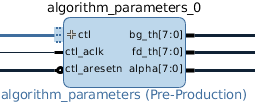
\includegraphics[]{img/algorithm-parameters.png}
	\caption{Graficzna reprezentacja modułu AXI DMA w programie Vivado.}
	\label{fig:axi-dma-diagram}
\end{figure}

Moduł wyposażony jest w interfejs AXI, podpisany \texttt{ctl} oraz związane z nim sygnały, zegarowy -- \texttt{ctl\_aclk} oraz reset -- \texttt{ctl\_aresetn}. 
Sygnały wyjściowe pozwalają na odczyt zdefiniowanych parametrów z poziomu innych modułów logiki reprogramowalnej. 
Dzięki wydzieleniu modułu odpowiedzialnego za konfigurację algorytmu z części wykonującej obliczenia algorytmiczne, możliwe jest uproszczenie kodu języka opisu sprzętu związanego z każdym z modułów oraz zwiększenie czytelności schematu. 
Jeden moduł konfiguracyjny może być związany z kilkoma, działającymi niezależnie, modułami algorytmicznymi. 
Ponadto, zmiany w strukturze algorytmu są uproszczone.
Proces projektowania oraz komunikacji z modułem przedstawiono w rozdziale \ref{sec:vivado-axi-dma}. 


\subsection{AXI Video DMA}
\label{sec:axi-vdma}
Interfejs AXI VDMA pozwala na wykorzystanie techniki DMA w przypadku aplikacji przetwarzających sygnał wizyjny.
Mechanizm \emph{Video DMA} oparty został na wykorzystaniu protokołu AXI w wersji Stream oraz Memory Mapped w połączeniu z techniką DMA do buforowania sygnału wizyjnego. 
Sygnał wizyjny przesyłany jest do modułu przy użyciu protokołu strumieniowego, gdzie następnie jest buforowany i zapisywany do komórek zewnętrznej pamięci RAM. 
Przechowywany obraz może być odczytany z poziomu procesora ARM.
Moduł wspiera również komunikację w drugą stronę, pozwalając na odczyt obrazu z pamięci i przesłanie go dalej w postaci strumienia. 
Połączenie tych technik pozwala na wykorzystanie modułu do buforowania obrazu lub w celu rozdzielenia zadań algorytmicznych pomiędzy FPGA i CPU.

Moduł VDMA pozwala na zdefiniowanie do trzydziestu dwóch buforów ramek obrazu. 
Operacje mogą być wykonywane cyklicznie na każdym buforze lub stale na jednym z nich. 
Pozwala to na wielokrotną transmisję jednej klatki obrazu.
Dane w buforze reprezentują kompletne ramki obrazu w ciągłym fragmencie pamięci, umożliwiając swobodny dostęp do poszczególnych pikseli. Struktura danych jest identyczna do tablicy zawierającej wartości kolejnych pikseli w obrazie.

Powszechnie wykorzystywanym zastosowaniem modułu jest mechanizm potrójnego buforowania, umożliwiający zmianę częstotliwości taktowania zegara sygnału wizyjnego. 
Zapis i odczyt danych może odbywać się niezależnie z tego samego lub różnych buforów. 
Dzięki zastosowaniu trzech buforów, zagwarantować można, że zapis i odczyt danych zawsze odbywa się z niezależnych obszarów pamięci, co pozwala uniknąć zjawiska nadpisania przechowywanych danych przed ich wyświetleniem.
W niniejszej pracy rozpatrzono możliwość wykorzystania modułu VDMA w celu obsługi algorytmów wymagających kontekstu w postaci dwóch kolejnych ramek obrazu.
Proces konfiguracji modułu przedstawiono w rozdziale \ref{sec:vivado-axi-vdma}.

\section{Obliczenia równoległe}
\label{sec:openmp}

Ze względu na wykorzystanie w układzie Zynq procesora ARM o dwóch rdzeniach, możliwe jest rozważenie zagadnienia zwiększania szybkości wykonania algorytmu przez zrówlnoleglenie obliczeń w dwóch wątkach. 
Stosując prawo Amdahla, wykazać można, że maksymalne przyspieszenie, jakie można uzyskać w systemie wieloprocesorowym jest proporcjonalne do liczby elementów obliczeniowych. 
Zależność ta zachodzi po warunkiem, że całe zadanie może być realizowane w sposób równoległy. 
W przypadku omawianego procesora, spodziewać się można korzyści nie przekraczających dwukrotnego zwiększenia szybkości wykonania algorytmu.

Zagadnienia związane z obliczeniami równoległymi stanowią obszar aktualnych badań, których efekty pozwoliły na zaprojektowanie zbioru bibliotek ułatwiających wykorzystanie własności systemów wieloprocesorowych w praktyce. 
W ramach pracy rozważono możliwości wykorzystania wątków natywnych oraz bibliotek Intel TBB(\emph{ang.} Threading Building Blocks) i OpenMP do budowy aplikacji wielowątkowych.

\subsection{Wątki natywne}

Użycie wątków natywnych wymaga wykorzystania bibliotek systemowych -- w przypadku aplikacji w języku C++ działającej w systemie PetaLinux zastosować można biblioteki \texttt{<thread>} lub \texttt{<pthread.h>} wchodzące w skład bibliotek standardowych \cite{Williams2013}.
Ich wykorzystanie pozwala na możliwie najbardziej efektywne użycie zasobów maszyny obliczeniowej. 
Wymaga to jednak dużych umiejętności programisty oraz dobrej znajomości architektury docelowej oraz wykonywanego zadania. 
Ponadto, zastosowanie biblioteki \texttt{<pthread.h>} wymaga zgodności systemu docelowego ze standardem POSIX, natomiast w przypadku \texttt{<thread>}, konieczne jest przeprowadzenie procesu kompilacji kompilatorem zgodnym ze standardem C++11. 
Założenia te mogą okazać się problematyczne w przypadku konieczności migracji aplikacji na system nie spełniający opisanych wymagań.

Stosowanie wątków natywnych pozwala na budowę wielowątkowych aplikacji działających heterogenicznie. 
Jest to najprostszy sposób na zbudowanie programu, w którym kilka wątków odpowiada za kilka różnych zadań. 
Na przykład, jeden wątek może być odpowiedzialny za przeprowadzenie obliczeń algorytmicznych, drugi za obsługę interfejsu użytkownika i przygotowanie danych wejściowych do właściwych obliczeń algorytmicznych, a kolejny -- za niekrytyczne operacje po zakończeniu pracy algorytmu, takie jak przesłanie wyników do bazy danych.

\subsection{Biblioteka Intel Threading Building Blocks}

Biblioteka Intel Threading Building Blocks stanowi zbiór narzędzi rozszerzających standard języka C++ o elementy związane z obliczeniami równoległymi. 
Składają się na to implementacje algorytmów równoległych, struktury danych przeznaczone do wykorzystania w systemach wielowątkowych oraz implementacje operacji atomowych i algorytmów wzajemnego wykluczania \cite{Reinders2010}.

Użycie biblioteki opiera się na zastosowaniu jej elementów na etapie powstawania aplikacji. 
Z tego względu, podobnie jak w przypadku wątków natywnych, konieczne jest zaprojektowanie aplikacji w sposób możliwie najlepiej wykorzystujący zalety biblioteki. 
Refaktoryzacja kodu istniejącego programu w taki sposób, by zastosować \emph{TBB} może być utrudniona i ostatecznie nie pozwolić na uzyskanie zadowalających wyników.


Główną zaletą stosowania \emph{TBB} jest większa skalowalność wynikowych rozwiązań. 
W przypadku zastosowania wątków natywnych, konieczne jest zaprojektowanie aplikacji w sposób umożliwiający wykorzystanie innej liczby wątków, gdy będzie to konieczne. 
W przypadku zastosowania dodatkowej biblioteki, stanowi ona warstwę abstrakcji pomiędzy programistą a warstwą obliczeniową, dzięki czemu proces możliwie najlepszej integracji aplikacji z platformą docelową odbywać się może przy niewielkiej interakcji ze strony projektanta.
Biblioteka \emph{TBB} zgodna jest z ideą programowania generycznego, paradygmatu powszechnie stosowanego w aplikacjach projektowanych w języku C++.
Jej stosowanie stanowi naturalne rozszerzenie możliwości tego języka i nie wymaga szerokiej wiedzy na temat architektury systemu docelowego.

\subsection{Biblioteka OpenMP}

Biblioteka OpenMP to interfejs programowania aplikacji pozwalający na budowanie wieloplatformowych programów wykonywanych równolegle. 
Rozwiązanie to jest dedykowane aplikacjom powstającym w językach C i C++ \cite{openmp-guide}.
OpenMP składa się z dyrektyw kompilatora i zbioru bibliotek, które pozwalają kształtować zachowanie programu na etapie wykonania. 
Ze względu na wykorzystanie dyrektyw kompilacji, możliwa jest integracja biblioteki z istniejącą aplikacją, nie wymagając przy tym modyfikowania właściwego kodu programu. 
Wymaga to wyłącznie znajomości aplikacji w stopniu umożliwiającym identyfikację obszarów, których równoległe wykonanie pozwoli na osiągnięcie największych zysków, obserwowanych w formie przyśpieszenia działania programu. 

Analogicznie jak w przypadku biblioteki \emph{TBB}, zastosowanie OpenMP ma na celu zapewnienie skalowalności aplikacji i dodanie warstwy abstrakcji pomiędzy kod programu, a operacje wykonywane na wątkach obliczeniowych. 
Obie biblioteki wyposażone są również w algorytmy równoważenia obciążenia.

Wykorzystanie biblioteki OpenMP wymaga zastosowania kompilatora wspierającego dyrektywy wchodzące w jej skład. 
Ze względu na specyfikę stosowania części interfejsu biblioteki -- w formie komentarzy do właściwego kodu aplikacji -- możliwa jest kompilacja programu kompilatorem nie wspierającym jej. 
Wynikowa aplikacja nie będzie korzystać z zalet przetwarzania równoległego, jednak powinna pozwalać na uzyskanie poprawnych wyników algorytmu.

\subsection*{Podsumowanie}

Trzy opisane rozwiązania zapewniają dostęp do różnych możliwości i obarczone są różnym kosztem stosowania. 
Z tego względu, nie jest możliwy jednoznaczny wybór najlepszego rozwiązania dla aplikacji wykonujących obliczenia równoległe. 
Często słuszne może okazać się wykorzystanie więcej niż jednej biblioteki w aplikacji, wykorzystując je do nadzoru nad zadaniami różnego typu. 
Część rozwiązań wymaga wsparcia kompilatora, część ograniczona jest do pewnej grupy systemów lub architektur. 
Wybór podejścia do obliczeń równoległych powinien stanowić etap projektowania aplikacji, a decyzja powinna uwzględniać szereg zagadnień.

W ramach pracy nie omówiono kilku innych popularnych rozwiązań związanych z obliczeniami wielowątkowymi, w tym \emph{OpenCL} oraz \emph{MPI}, ze względu na ograniczone możliwości ich wykorzystania w systemie PetaLinux działającym na platformie ZYBO.
Badane zagadnienie stanowi temat obszernych dyskusji, których wyniki odnaleźć można w publikowanych pracach \cite{choosing-thread-framework,Kegel2009}. 
W rozdziale \ref{sec:multithreading-config} opisano kroki wymagane do zastosowania omawianych bibliotek w aplikacjach uruchamianych w systemie PetaLinux.

%TODO A jakieś proste testy. Tak jak z tym neon - dałoby rady ?
% Hm... to rozwiązania programowe, niezależne od architektury, więc spodziewałbym się wyniku, w którym dla każdej metody uzyskaliśmy przyśpieszenie zbliżone do 2.
% Z TBB nie miałem okazji korzystać, ale spodziewałbym się, że "działa", pozostałe dwie metody znam dobrze (natywne) lub trochę (OMP) i, jeśli byłyby zauważalne różnice, to sądzę, że tylko dlatego, że gdzieś mógłbym popełnić błąd. :)
% To szeroki temat, wg. lepiej zostawić linki do szerszych źródeł, a testy pominąć, bo wyniki nie pokażą nic ciekawego.

%TODO OK.

\section{OpenCV}
\label{sec:opencv-lib}

Algorytmy wizyjne znajdują zastosowanie w wielu aplikacjach realizowanych w ramach projektów związanych z szerokim spektrum dziedzin techniki. 
Ze względu na swoją popularność, część rozwiązań została zintegrowana w zbiorze bibliotek OpenCV \cite{opencv-library}. 
Zbiór ten zawiera wydajne implementacje najczęściej stosowanych algorytmów, dedykowanych uruchamianiu na układach CPU oraz GPU (\emph{ang.} Graphics Processing Unit). 
Biblioteka jest szeroko stosowana ze względu na wysoką wydajność, stabilność działania i możliwość przenoszenia rozwiązań pomiędzy platformami o różnych architekturach.

Zastosowanie zewnętrznej biblioteki pozwala, w porównaniu do autorskiej implementacji algorytmu, na ograniczenie czasu wymaganego do zbudowania działającego prototypu. 
Ponadto, gotowe rozwiązania zapewniają zwykle większą stabilność i wystarczającą wydajność w większości przypadków. 
Kluczowym ograniczeniem względem autorskiej implementacji jest brak możliwości dostosowania algorytmu do rozpatrywanego przypadku. 
Może to wiązać się z koniecznością sprowadzenia danych wejściowych do struktury wspieranej przez bibliotekę, co może prowadzić do ograniczenia wydajności działania aplikacji.
Wśród algorytmów dostępnych w bibliotece znajdują się procedury detekcji i rozpoznawania twarzy, klasyfikacji zachowań, śledzenia obiektów, czy identyfikacji obrazów podobnych.

Wykorzystanie biblioteki OpenCV w aplikacjach \textit{bare-metal} może być niemożliwe ze względu na liczbę zależności, które należy dostarczyć do poprawnego jej działania. 
Dostępność systemu operacyjnego, takiego jak PetaLinux, pozwala na dołączenie do systemu plików bibliotek, wybierając je z puli prekompilowanych zasobów, dostępnych w pakiecie PetaLinux lub dostarczając zewnętrzny zbiór bibliotek, przygotowany przez użytkownika. 
Możliwości te zbadano w pracy na przykładzie biblioteki OpenCV w wersjach 2.4 oraz 3.1.

Pakiet PetaLinux oferuje dostęp do prekompilowanej biblioteki w wersji 3.1. 
Wydanie to wciąż znajduje się w początkowej fazie rozwoju i nie zostało w pełni zaadaptowane w części środowisk. 
Z tego powodu, wersja 2.4 biblioteki wciąż znajduje zastosowanie.
OpenCV w wersji 2.4 nie jest jednak oficjalnie dostępne w środowisku PetaLinux. 
Jego użycie wymaga zbudowania biblioteki na bazie kodu źródłowego wraz z zależnościami i dodanie plików wynikowych do zbioru bibliotek dostępnych w projekcie PetaLinux.
Przebieg procesu dla obu przypadków opisano w rozdziale \ref{sec:opencv-config}.

\section{Integracja algorytmów w FPGA i CPU}


Zagadnienie integracji rozwiązań algorytmicznych wewnątrz logiki programowalnej z obliczeniami prowadzonymi przez procesor ARM może pozwolić na zwiększenie wydajności działania aplikacji względem algorytmów realizowanych wyłącznie w jednym z tych układów.
Podział algorytmu na sekwencję etapów, realizowanych w logice reprogramowalnej lub w systemie procesorowym pozwala wykorzystać zalety obu rozwiązań. 
Układy FPGA pozwalają na użycie zbioru algorytmów w technice strumieniowej, co umożliwia dokonać przetwarzania obrazów w czasie rzeczywistym, z zachowaniem przyjętych opóźnień. 

Implementacja części algorytmów w sposób umożliwiający przetwarzanie strumieniowe może być niemożliwa. 
Procedury wymagające dużego kontekstu na etapie wykonania lub dostępu do danych historycznych projektowane są w celu uruchamiania na układach CPU o swobodnym dostępie do pamięci operacyjnej. 
Ponadto, realizacja algorytmów zdominowanych przez instrukcje lub wymagających zastosowania wyrażeń warunkowych i pętli może być nieefektywna w porównaniu do implementacji na CPU. 
Przykładami takich procedur mogą być śledzenie zmiennej liczby obiektów w kadrze czy stosunkowo proste operacje rotacji lub odbicia obrazu.

Podział algorytmu wizyjnego na etapy wykonywane naprzemiennie w logice programowalnej i procesorze ARM wymaga transmisji danych pomiędzy dwoma modułami. 
Realizacja tego zadania w obu kierunkach może być dokonana przy użyciu elementów AXI VDMA.
W ramach pracy, zbadano możliwość wykorzystania modułu VDMA do transmisji danych wizyjnych z poziomu FPGA do procesora ARM, w celu ich odczytu i prezentacji z wykorzystaniem komunikacji sieciowej.
Zbadano również możliwość konwersji danych do struktur dostępnych w bibliotece OpenCV, co umożliwia wykorzystanie biblioteki do realizacji algorytmów wizyjnych. 
Procedury odczytu oraz zapisu danych przedstawiono w dodatku \ref{sec:vdma-to-opencv}.

Sprawdzono szybkość działania procedur transmisji danych pomiędzy dwoma elementami obliczeniowymi dla sygnału wizyjnego o rozdzielczości HD ($1280 \times 720$ pikseli), przyjmując rozmiar piksela równy trzydziestu dwóm bitom w cyklu dziesięciu tysięcy iteracji odczytu i zapisu. Wyniki zebrano w tabeli \ref{tab:vdma-to-opencv}. Schemat komunikacji i wykorzystania pamięci w obu przypadkach przedstawiono na rysunkach \ref{fig:vdma-opencv-no-copy} i \ref{fig:vdma-opencv-with-copy}.

\begin{figure}[H]
	\centering
	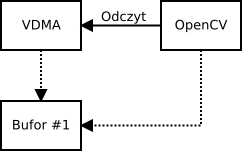
\includegraphics[height=4cm]{img/vdma-cv-comm-no-copy.pdf}
	\caption{Wymiana danych bez użycia procedur kopiowania.}
	\label{fig:vdma-opencv-no-copy}
\end{figure}

\begin{figure}[H]
	\centering
	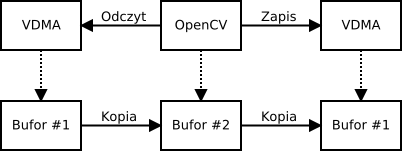
\includegraphics[height=4cm]{img/vdma-cv-comm-with-copy.pdf}
	\caption{Wymiana danych z wykorzystaniem procedur kopiowania.}
	\label{fig:vdma-opencv-with-copy}
\end{figure}

\begin{table}[H]
	\caption{Wyniki testu wydajnościowego transmisji danych.}
	\centering
	\label{tab:vdma-to-opencv}
\begin{tabular}{c|c|c|c|c|}
	\cline{2-5}
	& \multicolumn{2}{c|}{Bez kopiowania} & \multicolumn{2}{c|}{Z kopiowaniem} \\ \cline{2-5} 
	& Łącznie {[}s{]}  & Średnio {[}s{]}  & Łącznie {[}s{]}  & Średnio {[}s{]} \\ \hline
	\multicolumn{1}{|c|}{Odczyt} & $0,13$            & $0,000013$        & $151,34$           & $0,015$           \\ \hline
	\multicolumn{1}{|c|}{Zapis}  & ---              & ---              & $121,56$           & $0,012$           \\ \hline
\end{tabular}
\end{table}
%TODO napisać rozdzielczość w pikselech, jakie wyniki ?
% właściwie nie wiem, jak oszacować wydajność...
%TODO No ale napisał Pan "sprawdzono szybkość". No albo doprecyzować, albo przeregagować. Sam zapis do pamięci to pewnie działa real-time. Pytanie jak odczyt w ARM itp.
% dodałem wyniki zebrane w tabeli
Biblioteka OpenCV pozwala na użycie zewnętrznych źródeł danych do budowy struktur obrazu, a w konsekwencji pominąć etap kopiowania pamięci udostępnianej przez sterownik VDMA. 
W takim przypadku, czas odczytu pełnej ramki obrazu nie przekracza kilkunastu mikrosekund.
Należy jednak pamiętać, że stosując tę technikę, zagwarantować trzeba, że przetwarzanie obrazu zakończy się do chwili rozpoczęcia odczytu danych z wykorzystywanego bufora przez moduł VDMA. 
W przypadku zastosowania układu trzech buforów i sygnału wejściowego o częstotliwości sześćdziesięciu klatek na sekundę, daje to okno przetwarzania o długości szesnastu milisekund. 
Przekroczenie tej wartości może wpłynąć na błędną pracę algorytmu ze względu na nadpisanie danych przez moduł VDMA.

Z tego względu, rozważyć należy skopiowane danych wejściowych do nowego bufora na etapie odczytu oraz ponowne skopiowanie danych do bufora źródłowego w trakcie zapisu. 
Procedura odczytu wymaga średnio piętnastu milisekund, natomiast zapis zajmuje nie więcej niż dwanaście milisekund. 
Zastosowanie tej techniki nie pozwala na przetwarzanie sygnału wizyjnego w czasie rzeczywistym, gwarantuje jednak nienaruszalność danych. 
W połączeniu z zastosowaniem modułu VDMA o większej liczbie buforów, pozwala na integrację algorytmu o dużej złożoności obliczeniowej pomiędzy elementami obliczeniowymi obu typów. 
Jednakże, w celu zachowania limitów czasowych, konieczne może być ograniczenie przetwarzania danych do części klatek obrazu i pominięcie pozostałych. 
Nie powinno to jednak wpłynąć na zachowanie algorytmu wewnątrz logiki programowalnej.
%TODO no ale łąmie to ogranicze czasu czy nie...
%TODO trochę to niejasne. Może jakieś rysunek/schemat pokazujący oba podejscia ?
% wydaje mi się, że nie uda mi się przedstawić tego czytelniej niż w postaci kilku linii kodu w dodatki sec:vdma-to-opencv

% avg read = 0.000013, avg read_with_copy = 0.015134, avg write = 0.012156

%TODO OK, choć moim zdaniem rysunek dałoby się wyprodukować.
% hm... spróbowałem wykreować diagramy. O ile są czytelne, mogą zostać.
\section{Przerwania systemowe}
\label{sec:axi-interrupts}

Przerwanie to sygnał wysyłany przez urządzenie lub program, które ma na celu przekazanie do procesora informacji o zdarzeniu, które wymaga natychmiastowej obsługi.
Przerwania podzielić można na maskowalne i niemaskowalne. 
Klasa przerwań maskowalnych może być zdefiniowana jako ignorowana przez właściwe ustawienie rejestrów kontrolera przerwań. 
Druga klasa przerwań związana jest zwykle ze zdarzeniami o krytycznym znaczeniu, tak jak zdarzenia związane z działaniem zegarów czy układu \emph{watchdog}\footnote{Moduł odpowiedzialny za wykrycie błędnego działania systemu i wymuszający restart procesora w takiej sytuacji.}, więc ich wystąpienie nie może zostać zignorowane przez układ procesora. 

Wykorzystanie przerwań pozwala na zaprojektowanie interfejsu aplikacji współpracującej ze zbiorem urządzeń peryferyjnych, takich jak czujniki, przyciski, czy klawiatury. 
W przypadku układu Zynq, rolę urządzeń wysyłających sygnał przerwania przyjąć mogą również elementy logiki programowalnej, takie jak układy VDMA, zegary, czy moduły zaprojektowane przez użytkownika.

Układ Zynq wyposażony jest w moduł GIC (\emph{ang.} Generic Interrupt Controller), który pełni rolę kontrolera przerwań, odpowiedzialnego za obsługę zdarzeń. \emph{GIC} obsługuje przerwania z kilku źródeł:
\begin{itemize}
	\item przerwania programowe -- zbiór nie więcej niż szesnastu zdarzeń, które pozwalają na wywołanie procedury obsługi przerwania bezpośrednio z kodu aplikacji. Zachowanie to pozwala na komunikację z systemem operacyjnym i jest zwykle wykorzystywane do wywoływania operacji wejścia lub wyjścia. 
	
	Innym zastosowaniem przerwań programowych jest wysłanie sygnału \emph{yield}, który pozwala na dobrowolne wywłaszczenie obecnie aktywnego procesu przez układ planisty systemowego\footnote{Proces systemowy odpowiedzialny za wybór procesów do wykonania przez procesor w danej chwili. Wybrane zadania wykonywane są przez jednostkę przez ograniczony czas, po którym mogą został zatrzymane na rzecz innych oczekiwanych procesów.}. 
	
	\item przerwania systemowe -- współdzielone i prywatne -- zdarzenia zgłaszane przez sprzęt, na przykład klawiatury, moduły DMA czy układy pamięci. 
	Dla każdego urządzenia lub zbioru zdefiniowana jest unikalna linia przerwania, a do kategorii zdarzenia przypisany jest identyfikator. 
	Obsługa przerwania przez system operacyjny polega na wywołaniu agenta zdarzeń związanego z wyemitowanym identyfikatorem.
	
	Przerwania współdzielone pozwalają na komunikację pomiędzy procesorem a urządzeniami peryferyjnymi oraz układem FPGA, mogą być definiowane przez użytkownika i być obsługiwane przez dowolny rdzeń procesora. 
	Zdarzenia prywatne to przerwania definiowane niezależnie dla każdego rdzenia i pozwalają na obsługę zdarzeń zegarowych czy watchdoga.
\end{itemize}

W trakcie obsługi przerwania z dowolnego źródła, wykonanie kodu aplikacji jest wstrzymywane na czas wywołania kodu agenta obsługi zdarzenia. 
Stan rejestrów zapisywany jest na stosie i wykonywany jest kod odpowiedzialny za obsługę przerwania. 
Po zakończeniu wykonania, deklarowanego przez wywołanie instrukcji procesora \emph{RETI}, przywracany jest zapamiętany stan aplikacji i wznawiane jest jej wykonanie.

Przerwania to zdarzenia wywoływane asynchronicznie do normalnego działania aplikacji i mogące pochodzić z wielu źródeł, co może prowadzić do sytuacji, w której kilka linii przerwań sygnalizuje stan alarmu jednocześnie, co może powodować problemy z właściwą obsługą zdarzeń.
Procesor ARM pozwala na priorytetyzowanie przerwań. 
Przyznanie pierwszeństwa pewnemu zbiorowi krytycznych zdarzeń umożliwia rozwiązanie problemu kolejności wykonania w przypadku, gdy dwa zdarzenia o różnym priorytecie zostaną zgłoszone w tym samym czasie, a także na przerwanie obsługi przerwania o niskim priorytecie na rzecz wywołania agenta krytycznego zdarzenia.
Ze względu na charakter przerwań, część zdarzeń może mieć krytyczne znaczenie dla poprawnego wykonania aplikacji, a brak ich obsługi może prowadzić do zatrzymania działania procesora lub przeprowadzenia procesu restartu.

Procedury obsługi przerwań mogą być definiowane zarówno w aplikacjach typu \textit{bare-metal} jak i w systemach operacyjnych, takich jak PetaLinux.
Obsługa przerwań w aplikacji \textit{bare-metal} wymaga wykorzystania kontrolera do zarejestrowania agenta zdarzeń w formie funkcji aplikacji.

W przypadku systemu operacyjnego, konieczne jest wykorzystanie sterownika sprzętowego. 
W skład PetaLinux wchodzą sterowniki dedykowane zbiorowi modułów definiowanych w logice reprogramowalnej. 
Obsługa zdarzenia w niestandardowym module, zaprojektowanym przez użytkownika, wymagać może napisania dedykowanego sterownika urządzenia.
Zagadnienie to wykracza poza zakres niniejszej pracy i stanowi rozbudowany proces, wymagający szerokiej wiedzy na temat działania systemów operacyjnych. 
Temat ten omawiany jest w pracach \cite{Love2014,Corbet2005}.

W ramach pracy, zbadano możliwość wykorzystania przerwania emitowanego przez moduł AXI Timer, pozwalającego na wykonywanie operacji odliczania czasu oraz przerwań modułu AXI VDMA, pozwalających na przesłanie notyfikacji związanych ze zdarzeniami odczytu lub zapisu kolejnych ramek obrazu na właściwy im kanał.

Moduł AXI Timer wykorzystać można do odliczania czasu pomiędzy kolejnymi wykonaniami procedury, która powinna być wywoływania cyklicznie, w regularnych odstępach czasu. 
Działanie modułu AXI Timer może być warunkowane przez sygnały innych modułów logiki. 
Pozwala to na zaprojektowanie aplikacji, w której pewne zadanie wykonywane jest cyklicznie, pod warunkiem wystąpienia zdefiniowanego zdarzenia na poziomie logiki, a kontekst tego zdarzenia nie musi być znany z poziomu aplikacji wykonywanej przez procesor -- na przykład, wykonanie przez aplikację operacji analizy danych uzyskiwanych przez algorytm wizyjny cyklicznie, pod warunkiem, że moduł algorytmu wykonywany przez układ logiczny ustawił sygnał spójności wyników.
Podobne zachowanie uzyskać można korzystając z funkcji procesora i związanych z nim zegarów, co ogranicza jednak możliwości konfiguracji działania procedury do kontekstu znanego z poziomu CPU.


Przerwania definiowane przez moduł AXI VDMA pozwalają na zgłoszenie zdarzenia po wykonaniu procesu odczytu lub zapisu określonej liczby ramek obrazu lub po upływie określonego czasu od uzyskania sygnałów synchronizacji obrazu. 
Wykorzystanie tych mechanizmów pozwala na zaprojektowanie procedur aplikacji, które powinny być wykonane co określoną liczbę klatek sygnału wizyjnego. 
W szczególnym przypadku, mechanizm ten pozwala na wykonanie przez procesor dla każdej ramki obrazu operacji algorytmicznych, których implementacja sprzętowa byłaby trudna lub niemożliwa. 
Mechanizm ten pozwala również na przeprowadzenie operacji końcowej analizy wyników algorytmu wizyjnego, zaimplementowanego w logice programowalnej. 
Proces konfiguracji projektu wykorzystującego mechanizm przerwań opisano w rozdziale \ref{sec:interrupts-config}.